% GNUPLOT: LaTeX picture with Postscript
\begingroup
  \makeatletter
  \providecommand\color[2][]{%
    \GenericError{(gnuplot) \space\space\space\@spaces}{%
      Package color not loaded in conjunction with
      terminal option `colourtext'%
    }{See the gnuplot documentation for explanation.%
    }{Either use 'blacktext' in gnuplot or load the package
      color.sty in LaTeX.}%
    \renewcommand\color[2][]{}%
  }%
  \providecommand\includegraphics[2][]{%
    \GenericError{(gnuplot) \space\space\space\@spaces}{%
      Package graphicx or graphics not loaded%
    }{See the gnuplot documentation for explanation.%
    }{The gnuplot epslatex terminal needs graphicx.sty or graphics.sty.}%
    \renewcommand\includegraphics[2][]{}%
  }%
  \providecommand\rotatebox[2]{#2}%
  \@ifundefined{ifGPcolor}{%
    \newif\ifGPcolor
    \GPcolortrue
  }{}%
  \@ifundefined{ifGPblacktext}{%
    \newif\ifGPblacktext
    \GPblacktextfalse
  }{}%
  % define a \g@addto@macro without @ in the name:
  \let\gplgaddtomacro\g@addto@macro
  % define empty templates for all commands taking text:
  \gdef\gplbacktext{}%
  \gdef\gplfronttext{}%
  \makeatother
  \ifGPblacktext
    % no textcolor at all
    \def\colorrgb#1{}%
    \def\colorgray#1{}%
  \else
    % gray or color?
    \ifGPcolor
      \def\colorrgb#1{\color[rgb]{#1}}%
      \def\colorgray#1{\color[gray]{#1}}%
      \expandafter\def\csname LTw\endcsname{\color{white}}%
      \expandafter\def\csname LTb\endcsname{\color{black}}%
      \expandafter\def\csname LTa\endcsname{\color{black}}%
      \expandafter\def\csname LT0\endcsname{\color[rgb]{1,0,0}}%
      \expandafter\def\csname LT1\endcsname{\color[rgb]{0,1,0}}%
      \expandafter\def\csname LT2\endcsname{\color[rgb]{0,0,1}}%
      \expandafter\def\csname LT3\endcsname{\color[rgb]{1,0,1}}%
      \expandafter\def\csname LT4\endcsname{\color[rgb]{0,1,1}}%
      \expandafter\def\csname LT5\endcsname{\color[rgb]{1,1,0}}%
      \expandafter\def\csname LT6\endcsname{\color[rgb]{0,0,0}}%
      \expandafter\def\csname LT7\endcsname{\color[rgb]{1,0.3,0}}%
      \expandafter\def\csname LT8\endcsname{\color[rgb]{0.5,0.5,0.5}}%
    \else
      % gray
      \def\colorrgb#1{\color{black}}%
      \def\colorgray#1{\color[gray]{#1}}%
      \expandafter\def\csname LTw\endcsname{\color{white}}%
      \expandafter\def\csname LTb\endcsname{\color{black}}%
      \expandafter\def\csname LTa\endcsname{\color{black}}%
      \expandafter\def\csname LT0\endcsname{\color{black}}%
      \expandafter\def\csname LT1\endcsname{\color{black}}%
      \expandafter\def\csname LT2\endcsname{\color{black}}%
      \expandafter\def\csname LT3\endcsname{\color{black}}%
      \expandafter\def\csname LT4\endcsname{\color{black}}%
      \expandafter\def\csname LT5\endcsname{\color{black}}%
      \expandafter\def\csname LT6\endcsname{\color{black}}%
      \expandafter\def\csname LT7\endcsname{\color{black}}%
      \expandafter\def\csname LT8\endcsname{\color{black}}%
    \fi
  \fi
    \setlength{\unitlength}{0.0500bp}%
    \ifx\gptboxheight\undefined%
      \newlength{\gptboxheight}%
      \newlength{\gptboxwidth}%
      \newsavebox{\gptboxtext}%
    \fi%
    \setlength{\fboxrule}{0.5pt}%
    \setlength{\fboxsep}{1pt}%
\begin{picture}(7200.00,5040.00)%
    \gplgaddtomacro\gplbacktext{%
    }%
    \gplgaddtomacro\gplfronttext{%
      \csname LTb\endcsname%
      \put(6671,309){\makebox(0,0)[l]{\strut{}}}%
      \csname LTb\endcsname%
      \put(6671,399){\makebox(0,0)[l]{\strut{}}}%
      \csname LTb\endcsname%
      \put(6671,490){\makebox(0,0)[l]{\strut{}}}%
      \csname LTb\endcsname%
      \put(6671,580){\makebox(0,0)[l]{\strut{}}}%
      \csname LTb\endcsname%
      \put(6671,670){\makebox(0,0)[l]{\strut{}}}%
      \csname LTb\endcsname%
      \put(6671,760){\makebox(0,0)[l]{\strut{}}}%
      \csname LTb\endcsname%
      \put(6671,850){\makebox(0,0)[l]{\strut{}}}%
      \csname LTb\endcsname%
      \put(6671,941){\makebox(0,0)[l]{\strut{}}}%
      \csname LTb\endcsname%
      \put(6671,1031){\makebox(0,0)[l]{\strut{}}}%
      \csname LTb\endcsname%
      \put(6671,1121){\makebox(0,0)[l]{\strut{}}}%
      \csname LTb\endcsname%
      \put(6671,1211){\makebox(0,0)[l]{\strut{}}}%
      \csname LTb\endcsname%
      \put(6671,1302){\makebox(0,0)[l]{\strut{}}}%
      \csname LTb\endcsname%
      \put(6671,1392){\makebox(0,0)[l]{\strut{}}}%
      \csname LTb\endcsname%
      \put(6671,1482){\makebox(0,0)[l]{\strut{}}}%
      \csname LTb\endcsname%
      \put(6671,1572){\makebox(0,0)[l]{\strut{}}}%
      \csname LTb\endcsname%
      \put(6671,1662){\makebox(0,0)[l]{\strut{}}}%
      \csname LTb\endcsname%
      \put(6671,1753){\makebox(0,0)[l]{\strut{}}}%
      \csname LTb\endcsname%
      \put(6671,1843){\makebox(0,0)[l]{\strut{}}}%
      \csname LTb\endcsname%
      \put(6671,1933){\makebox(0,0)[l]{\strut{}}}%
      \csname LTb\endcsname%
      \put(6671,2023){\makebox(0,0)[l]{\strut{}}}%
      \csname LTb\endcsname%
      \put(6671,2114){\makebox(0,0)[l]{\strut{}}}%
      \csname LTb\endcsname%
      \put(6671,2204){\makebox(0,0)[l]{\strut{}}}%
      \csname LTb\endcsname%
      \put(6671,2294){\makebox(0,0)[l]{\strut{}}}%
      \csname LTb\endcsname%
      \put(6671,2384){\makebox(0,0)[l]{\strut{}}}%
      \csname LTb\endcsname%
      \put(6671,2474){\makebox(0,0)[l]{\strut{}}}%
      \csname LTb\endcsname%
      \put(6671,2565){\makebox(0,0)[l]{\strut{}}}%
      \csname LTb\endcsname%
      \put(6671,2655){\makebox(0,0)[l]{\strut{}}}%
      \csname LTb\endcsname%
      \put(6671,2745){\makebox(0,0)[l]{\strut{}}}%
      \csname LTb\endcsname%
      \put(6671,2835){\makebox(0,0)[l]{\strut{}}}%
      \csname LTb\endcsname%
      \put(6671,2925){\makebox(0,0)[l]{\strut{}}}%
      \csname LTb\endcsname%
      \put(6671,3016){\makebox(0,0)[l]{\strut{}}}%
      \csname LTb\endcsname%
      \put(6671,3106){\makebox(0,0)[l]{\strut{}}}%
      \csname LTb\endcsname%
      \put(6671,3196){\makebox(0,0)[l]{\strut{}}}%
      \csname LTb\endcsname%
      \put(6671,3286){\makebox(0,0)[l]{\strut{}}}%
      \csname LTb\endcsname%
      \put(6671,3377){\makebox(0,0)[l]{\strut{}}}%
      \csname LTb\endcsname%
      \put(6671,3467){\makebox(0,0)[l]{\strut{}}}%
      \csname LTb\endcsname%
      \put(6671,3557){\makebox(0,0)[l]{\strut{}}}%
      \csname LTb\endcsname%
      \put(6671,3647){\makebox(0,0)[l]{\strut{}}}%
      \csname LTb\endcsname%
      \put(6671,3737){\makebox(0,0)[l]{\strut{}}}%
      \csname LTb\endcsname%
      \put(6671,3828){\makebox(0,0)[l]{\strut{}}}%
      \csname LTb\endcsname%
      \put(6671,3918){\makebox(0,0)[l]{\strut{}}}%
      \csname LTb\endcsname%
      \put(6671,4008){\makebox(0,0)[l]{\strut{}}}%
      \csname LTb\endcsname%
      \put(6671,4098){\makebox(0,0)[l]{\strut{}}}%
      \csname LTb\endcsname%
      \put(6671,4189){\makebox(0,0)[l]{\strut{}}}%
      \csname LTb\endcsname%
      \put(6671,4279){\makebox(0,0)[l]{\strut{}}}%
      \csname LTb\endcsname%
      \put(6671,4369){\makebox(0,0)[l]{\strut{}}}%
      \csname LTb\endcsname%
      \put(6671,4459){\makebox(0,0)[l]{\strut{}}}%
      \csname LTb\endcsname%
      \put(6671,4549){\makebox(0,0)[l]{\strut{}}}%
      \csname LTb\endcsname%
      \put(6671,4640){\makebox(0,0)[l]{\strut{}}}%
      \csname LTb\endcsname%
      \put(6671,4730){\makebox(0,0)[l]{\strut{}}}%
      \csname LTb\endcsname%
      \put(392,4775){\makebox(0,0){\strut{}}}%
      \csname LTb\endcsname%
      \put(516,4775){\makebox(0,0){\strut{}}}%
      \csname LTb\endcsname%
      \put(640,4775){\makebox(0,0){\strut{}}}%
      \csname LTb\endcsname%
      \put(765,4775){\makebox(0,0){\strut{}}}%
      \csname LTb\endcsname%
      \put(889,4775){\makebox(0,0){\strut{}}}%
      \csname LTb\endcsname%
      \put(1013,4775){\makebox(0,0){\strut{}}}%
      \csname LTb\endcsname%
      \put(1137,4775){\makebox(0,0){\strut{}}}%
      \csname LTb\endcsname%
      \put(1261,4775){\makebox(0,0){\strut{}}}%
      \csname LTb\endcsname%
      \put(1386,4775){\makebox(0,0){\strut{}}}%
      \csname LTb\endcsname%
      \put(1510,4775){\makebox(0,0){\strut{}}}%
      \csname LTb\endcsname%
      \put(1634,4775){\makebox(0,0){\strut{}}}%
      \csname LTb\endcsname%
      \put(1758,4775){\makebox(0,0){\strut{}}}%
      \csname LTb\endcsname%
      \put(1882,4775){\makebox(0,0){\strut{}}}%
      \csname LTb\endcsname%
      \put(2006,4775){\makebox(0,0){\strut{}}}%
      \csname LTb\endcsname%
      \put(2131,4775){\makebox(0,0){\strut{}}}%
      \csname LTb\endcsname%
      \put(2255,4775){\makebox(0,0){\strut{}}}%
      \csname LTb\endcsname%
      \put(2379,4775){\makebox(0,0){\strut{}}}%
      \csname LTb\endcsname%
      \put(2503,4775){\makebox(0,0){\strut{}}}%
      \csname LTb\endcsname%
      \put(2627,4775){\makebox(0,0){\strut{}}}%
      \csname LTb\endcsname%
      \put(2752,4775){\makebox(0,0){\strut{}}}%
      \csname LTb\endcsname%
      \put(2876,4775){\makebox(0,0){\strut{}}}%
      \csname LTb\endcsname%
      \put(3000,4775){\makebox(0,0){\strut{}}}%
      \csname LTb\endcsname%
      \put(3124,4775){\makebox(0,0){\strut{}}}%
      \csname LTb\endcsname%
      \put(3248,4775){\makebox(0,0){\strut{}}}%
      \csname LTb\endcsname%
      \put(3372,4775){\makebox(0,0){\strut{}}}%
      \csname LTb\endcsname%
      \put(3497,4775){\makebox(0,0){\strut{}}}%
      \csname LTb\endcsname%
      \put(3621,4775){\makebox(0,0){\strut{}}}%
      \csname LTb\endcsname%
      \put(3745,4775){\makebox(0,0){\strut{}}}%
      \csname LTb\endcsname%
      \put(3869,4775){\makebox(0,0){\strut{}}}%
      \csname LTb\endcsname%
      \put(3993,4775){\makebox(0,0){\strut{}}}%
      \csname LTb\endcsname%
      \put(4117,4775){\makebox(0,0){\strut{}}}%
      \csname LTb\endcsname%
      \put(4242,4775){\makebox(0,0){\strut{}}}%
      \csname LTb\endcsname%
      \put(4366,4775){\makebox(0,0){\strut{}}}%
      \csname LTb\endcsname%
      \put(4490,4775){\makebox(0,0){\strut{}}}%
      \csname LTb\endcsname%
      \put(4614,4775){\makebox(0,0){\strut{}}}%
      \csname LTb\endcsname%
      \put(4738,4775){\makebox(0,0){\strut{}}}%
      \csname LTb\endcsname%
      \put(4863,4775){\makebox(0,0){\strut{}}}%
      \csname LTb\endcsname%
      \put(4987,4775){\makebox(0,0){\strut{}}}%
      \csname LTb\endcsname%
      \put(5111,4775){\makebox(0,0){\strut{}}}%
      \csname LTb\endcsname%
      \put(5235,4775){\makebox(0,0){\strut{}}}%
      \csname LTb\endcsname%
      \put(5359,4775){\makebox(0,0){\strut{}}}%
      \csname LTb\endcsname%
      \put(5483,4775){\makebox(0,0){\strut{}}}%
      \csname LTb\endcsname%
      \put(5608,4775){\makebox(0,0){\strut{}}}%
      \csname LTb\endcsname%
      \put(5732,4775){\makebox(0,0){\strut{}}}%
      \csname LTb\endcsname%
      \put(5856,4775){\makebox(0,0){\strut{}}}%
      \csname LTb\endcsname%
      \put(5980,4775){\makebox(0,0){\strut{}}}%
      \csname LTb\endcsname%
      \put(6104,4775){\makebox(0,0){\strut{}}}%
      \csname LTb\endcsname%
      \put(6229,4775){\makebox(0,0){\strut{}}}%
      \csname LTb\endcsname%
      \put(6353,4775){\makebox(0,0){\strut{}}}%
      \csname LTb\endcsname%
      \put(6477,4775){\makebox(0,0){\strut{}}}%
    }%
    \gplbacktext
    \put(0,0){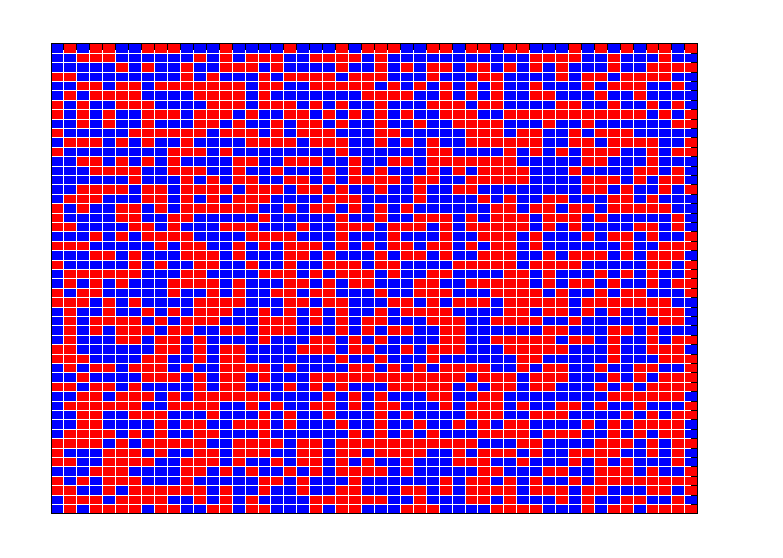
\includegraphics{grid}}%
    \gplfronttext
  \end{picture}%
\endgroup
